\documentclass[t]{beamer}
\usetheme{Warsaw}
\usepackage{array}
%\usepackage{graphicx}
\usepackage{amssymb,amsmath,mathrsfs,amsfonts}
%\usepackage[colorhighlight,display]{texpower}
%\usepackage{caption}
%\usepackage[all]{xy}
\usepackage{beamerthemesplit}
\mode<presentation>
%\usepackage{pause}
\usepackage{ulem}  % for strikethroughs
\usepackage{cancel} % for strikethroughs in math mode 
\usepackage{tikz}
\usetikzlibrary{shapes}
\usepackage{hyperref}
\hypersetup{pdfpagemode=FullScreen}
\usepackage{ifthen}
\usepackage{animate}
\usepackage{color}
\usepackage{type1cm}  % used for watermarking
\usepackage{eso-pic}  % used for watermarking


\theoremstyle{plain}
\newtheorem{prop}{Proposition}
\newtheorem{thm}[prop]{Theorem}
\newtheorem{lem}[prop]{Lemma}
\newtheorem{cor}[prop]{Corollary}
\theoremstyle{definition}
\newtheorem{dfn}{Definition}
\newtheorem{rem}[prop]{Remark}
\newtheorem{ex}{Example}[section]
%\newtheorem{note}{Note}[section]
\newtheorem{exercise}{Exercise}[section]
\newcommand{\nin}{\noindent}
\newcommand{\ds}{\displaystyle}
\renewcommand{\figurename}{Figure \arabic{figure}}



\renewcommand*\familydefault{\sfdefault} 




%%%%%%%%%%%%%%%%%%%%%%%%%%5
%%%%%%%%%%%%%%%%%%%%%%%%%%%%
%%%% some commands that have different meaning in the article/presentation modes

\newcommand{\vvfill}{\mode<presentation>{\vfill}  \mode<article>{\medskip}}   %vfill in presentation only
\newcommand{\sketchspace}{ 
\mode<article>{ \medskip\noindent{\textbf{Sketch:}} \vspace*{6cm} }
\mode<presentation>{ } 
}
\newcommand{\examplespace}{ 
\mode<article>{ \medskip\noindent{\textbf{Example:}} \vspace{6cm} }
\mode<presentation>{ } 
}
\newcommand{\artsmspace}{\mode<article>{\vspace*{2cm}} }  %small space in article mode
\newcommand{\artlargespace}{\mode<article>{\vspace*{6cm}} }  %large space in article mode

\newcommand{\dx}{\,dx}

\newcommand{\soln}{{\textbf{Solution: }}\,\,\,}
\newcommand{\disp}{\displaystyle}

\newcommand{\makedate}{\vvfill
\begin{picture}(10,10)  
\put(260,-20){\mbox{\tiny{\today}}}
\end{picture}
}

\newcommand{\pd}[2]{\dfrac{\partial#1}{\partial#2}}
\newcommand{\pD}[2]{\dfrac{\partial^2#1}{\partial#2^2}}
\newcommand{\pdd}[3]{\dfrac{\partial^2#1}{\partial#2 \partial#3}}


\normalem %stops the ulem package making all the emphs into underlines....
 
 
 
 \newcommand{\refandrev}[2]{
 \begin{small}
  \hspace{6cm}
  \begin{minipage}[r]{8cm}
  Stewart,    Chapter #1   \\
  Review:  \parbox[t]{6cm}{#2}
\end{minipage}
\end{small}
}



\newcounter{heading}
\setcounter{section}{1}
\setcounter{heading}{0}

\newcommand{\makeheading}[1]{\medskip\begin{large}\noindent\textbf{{#1}}\end{large}\smallskip}

%\newenvironment{head}[1]{\medskip\stepcounter{heading}\noindent\textbf{\hspace{0.2cm}{#1}.}}{}
\newcommand{\newhead}[1]{\medskip\stepcounter{heading}\noindent\textbf{\hspace{0.2cm}{#1}.}}


\newcommand{\pf}[1]{\noindent\textit{Proof.}\vspace*{#1 cm}}
\newcommand{\sol}[1]{\noindent\textit{Solution.}\vspace*{#1 cm}}
\newcommand{\further}[1]{\begin{small}\noindent\textit{Further reading: #1}\end{small}}
\newcommand{\exr}[1]{\begin{footnotesize}\noindent\textit{\textbf{Exercises:} Stewart #1}\end{footnotesize}}


% Sets of numbers
\newcommand{\C}{\mathbb{C}}
\newcommand{\RR}{\mathbb{R}}
\newcommand{\Z}{\mathbb{Z}}
\newcommand{\N}{\mathbb{N}}
\newcommand{\Q}{\mathbb{Q}}

% Partitions
\newcommand{\PP}{\mathcal{P}}

% Limits
\newcommand{\limm}[1]{\displaystyle \lim_{x\to #1}}

% Backslash
\newcommand{\bs}{\backslash}

% functions
\newcommand{\cosec}{\mathrm{cosec}}
\newcommand{\cosech}{\mathrm{cosech}}
\newcommand{\sech}{\mathrm{sech}}
\newcommand{\Li}{\mathrm{Li}}
\newcommand{\si}{\mathrm{Si}}
\newcommand{\erf}{\mathrm{erf}}

% Domain and Range
\newcommand{\Dom}{\mathrm{Dom}}
\newcommand{\Codom}{\mathrm{Codom}}
\newcommand{\Range}{\mathrm{Ran}}



\title{Week 3:  Limits, continuity, derivatives of functions}
\date{July 6 -- August 10, 2012}

\begin{document}

\frame{\titlepage}

\setcounter{tocdepth}{2}
\frame{\tableofcontents

\begin{flushright}
\hyperlink{tues}{\beamergotobutton{Lecture 6}}
\end{flushright} 
}

\AtBeginSection[]
{
\begin{frame}<beamer> 
\tableofcontents[currentsection]  % show TOC and highlight current section
\end{frame}
}

%\section*{Limits at infinity}
\begin{frame}
\newhead{Indeterminate forms}

\uncover<+->{\noindent Limits of the type
\[\limm{\infty}\frac{f(x)}{g(x)}\]
where $f(x)\to\infty$ and $g(x)\to\infty$ as $x\to\infty$ are said to be limits of the form $\frac{\infty}{\infty}$.}
\uncover<+->{While the following limits have the form $\frac{\infty}{\infty}$, each displays very different limiting behavior as $x\to\infty$:}
\begin{itemize}[<+->]
\item $\qquad$ $\limm{\infty}\frac{x}{x}$
\item $\qquad$ $\limm{\infty}\frac{x}{x^{2}}$
\item $\qquad$ $\limm{\infty}\frac{x^{3}}{x}$
\item $\qquad$ $\limm{\infty}\frac{e^{x}}{x}$ $\qquad$ (deal with this more later)
\end{itemize}

\end{frame}

\begin{frame}
\uncover<+->{Since we cannot determine in advance what kind of limiting behavior something of the form $\frac{\infty}{\infty}$ has, we say that $\frac{\infty}{\infty}$ is an \textit{indeterminate form}.  Note that $\infty-\infty$ and $\frac{0}{0}$ are also indeterminate forms. }

\uncover<+->{\newhead{Limits of the form $f(x)/g(x)$}
To calculate a limit of the form
\[\limm{\infty}\frac{f(x)}{g(x)}\]
where both $f(x)$ and $g(x)$ tend to infinity as $x\to\infty$, one approach is to divide both $f$ and $g$ by the \textit{fastest growing term} appearing in the denominator $g$.}

\uncover<+->{\newhead{Examples} }
\begin{enumerate}[<+->]
\item Evaluate $\limm{\infty}\frac{3x^2-x+1}{7+6x^2}$.
\item Find $\limm{\infty}\frac{x^2+3x}{\sqrt{2x^4+3}-4x}$.
\end{enumerate} 
\end{frame}

\begin{frame}
\newhead{Limits of the form $\sqrt{f(x)}-\sqrt{g(x)}$} The trick is to multiply both numerator and denominator by the `conjugate squared,' and then expand the numerator as a difference of squares.\pause


\vspace*{.4cm}

\newhead{Example}
Evaluate $\limm{\infty}\big(\sqrt{x^2+x}-x\big)$, if it exists.

\end{frame}

\section{Continuity}
\subsection{Continuous functions}
\begin{frame}
\frametitle{Continuous functions}
\begin{small}
\uncover<+->{\noindent Many quantities that occur in nature and change with time vary in a `continuous' manner; that is, they are not subject to interruption or abrupt change. For example, suppose that $f(t)$ denotes}
\begin{itemize}[<+->]
\item the distance from the sun to the earth at time $t$, or
\item the temperature at the back of the lecture theatre at time $t$.
\end{itemize}

\uncover<+->{Then $f$ has the property that a sufficiently small change in $t$ will  produce a small change in $f(t)$. Such a function $f$ is said to be `continuous'.  This intuitive notion is formalized in the following sequence of definitions.}
\end{small}


\uncover<+->{\begin{dfn} Suppose that $f$ is defined on some open interval containing the point $a$. If
\[\limm{a}f(x) = f(a) \]
then we say that $f$ is \textit{continuous} at $a$; otherwise, we say that $f$ is \textit{discontinuous} at $a$.\end{dfn}}
\end{frame}

\begin{frame}
\frametitle{Continuous functions}
\uncover<+->{\newhead{True or False: the following functions are continuous at the indicated point:}}
\begin{enumerate}[<+->]
\item $f(x) = x^{2}, \qquad a = 2.$
\vspace*{.4cm}

\item $f(x) = ln(x), \qquad a = -1.$
\vspace*{.4cm}

\item $f(x) = \begin{cases}
x^{2} &\mbox{if $x\leq 3$}\\
1&\mbox{if $x > 3$,}
\end{cases}, \qquad a = 3$
\vspace*{.4cm}

\item $f(x) = \begin{cases}
x^{2} &\mbox{if $x\neq 3$}\\
1&\mbox{if $x = 3$,}
\end{cases}, \qquad a = 3$


\end{enumerate}
\end{frame}

\begin{frame}
\frametitle{Continuous functions}
\uncover<+->{\noindent We have defined continuity at a point; now we define continuity on intervals.}

\uncover<+->{\newhead{Definition} Suppose that $f$ is a real-valued function defined on an open interval $(a,b)$. We say that $f$ is a \textit{continuous on $(a,b)$} if $f$ is continuous at every point in the interval $(a,b)$.}

\uncover<+->{\newhead{True or False?} $f(x) = \frac{1}{x}$ is continuous on $(0,1)$.}

\uncover<+->{\newhead{Definition} Suppose that $f$ is a real-valued function\\ defined on a closed interval $[a,b]$. We say that
\begin{enumerate}
\item[(a)] $f$ is continuous at the endpoint $a$ if $\limm{a^+}f(x)=f(a)$,
\item[(b)] $f$ is continuous at the endpoint $b$ if $\limm{b^-}f(x)=f(b)$,
\item[(c)] $f$ is continuous on the closed interval $[a,b]$ if $f$ is continuous on the open interval $(a,b)$ and at each of the endpoints $a$ and $b$.
\end{enumerate}}

\end{frame}

\begin{frame}
\frametitle{Continuous functions}
\uncover<+->{\newhead{True or False?}}

\begin{enumerate}[<+->]
\item $f(x) = \frac{1}{x}$ is continuous on $[1, 2]$
\item $f(x) = \frac{1}{x}$ is not continuous on $[0,1]$.
\end{enumerate}


\uncover<+->{\newhead{Definition} A function $f$ is said to be \textit{continuous} (or \textit{continuous everywhere}) if it is continuous at every point $a$ of its domain.}
\vspace*{.4cm}

\uncover<+->{\newhead{True or False?} $f(x) = x^2$ is continuous everywhere.}
\end{frame}

\begin{frame}
\frametitle{Discontinuities} A discontinuity can be further classified as a removable, jump or infinite discontinuity.

\begin{enumerate}[<+->]
\item[(i)] $f(x) = \frac{x^{2} - x - 2}{x -2}$ has a removable discontinuity at $x = 2$.
\vspace*{.4 cm}
\item[(ii)] $f(x) = \frac{1}{x}$ has an infinite discontinuity at $x = 0$.
\vspace*{.4 cm}
\item[(iii)] $f(x) = \begin{cases}
x^{2} &\mbox{if $x\leq 3$}\\
1&\mbox{if $x > 3$,}
\end{cases}$ has a jump discontinuity at $x = 3$.
\end{enumerate}
\end{frame}

\begin{frame}
\frametitle{Combining continuous functions}

\uncover<+->{\begin{prop} Suppose that the functions $f$ and $g$ are continuous at a point $a$. Then $f+g$, $f-g$ and $fg$ are continuous at $a$. If $g(a)\neq0$ then $f/g$ is also continuous at $a$.\end{prop}}



\uncover<+->{\begin{prop} Suppose that $f$ is continuous at $a$ and that $g$ is continuous at $f(a)$. Then $g\circ f$ is continuous at $a$.\end{prop}}

\uncover<+->{\begin{cor} Suppose that $f$ and $g$ are continuous on their domains and that $\limm{a}f(x)$ belongs to $\Dom(g)$. Then\vspace*{-.4 cm}
\[\vspace*{-.4 cm}\limm{a}g(f(x))=g\big(\limm{a}f(x)\big).\]
(\emph{``you can move limits inside continuous functions''})\end{cor}}
\end{frame}

\begin{frame}
\frametitle{Combining continuous functions}

\newhead{Example} Suppose that $a$ and $b$ are real numbers and consider the function $f$ with domain $\RR$ given by
\[
f(x)=
\begin{cases}
x^2-a^2&\mbox{if }x<0\\
\cos x+b &\mbox{if }x\geq0.
\end{cases}
\]
For what values of $a$ and $b$ will $f$ be continuous at $0$?
\end{frame}

\subsection{The intermediate value theorem}
\begin{frame}[label=tues]
\frametitle{The intermediate value theorem (IVT)}

\uncover<+->{
\begin{theorem}[The intermediate value theorem] 
Suppose that $f$ is continuous on the closed interval $[a,b]$. If $z$ lies between $f(a)$ and $f(b)$ then there is at least one real number $c$ in $[a,b]$ such that $f(c)=z$.
\end{theorem}}




\uncover<+->{\newhead{Example} Show that the equation
\[e^x=3\cos x -1\]
has at least one positive solution.}
\end{frame}

\section{Derivatives}
\subsection{Meaning and Computation of derivatives}

\frame
{
\frametitle{Average rate of change}
\begin{dfn}
\[ \text{Average rate of change of }f(x)\,=\frac{\text{Change in }y=f(x)}{\text{Change in }x} \]
\end{dfn}\pause
That is, \begin{dfn}
\begin{multline*} \text{Average rate of change of }f(x)\text{ between }x=a\text{ and }x=b\\=\frac{f(b)-f(a)}{b-a}\\
\pause
=\text{ Slope of the line passing through the points }(a,f(a))\\\text{ and }(b,f(b)).
\end{multline*} 
\end{dfn}
}

\frame
{
\frametitle{Average rate of change}
Let us look at an example:
\begin{figure}[t]
\begin{center}
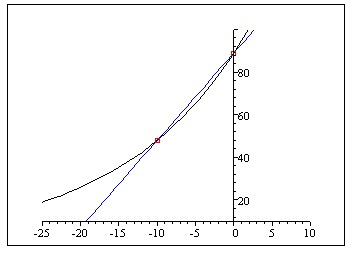
\includegraphics[scale=0.4]{image011.jpg}
\caption{Graph of $f(x)$ between $x=-10$ and $x=0$.}
\label{fig:3}
\end{center}
\end{figure}\pause

\nin Average rate of change of $f(x)$ between $x=-10$ and $x=0$\pause
\[ =\frac{f(0)-f(-10)}{(0-(-10))}
=\frac{88-48}{10}=\frac{40}{10}=4. \]
}

\frame
{
\frametitle{Average rate of change}
\begin{figure}[t]
\begin{center}
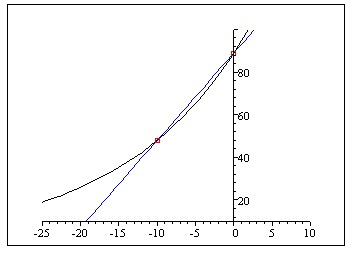
\includegraphics[scale=0.4]{image011.jpg}
\end{center}
\end{figure}

Note that, \\ Average rate of change of $f(x)$ between $x=-10$ and $x=0$ \\ \pause
 $=$ Slope of the secant line joining $(-10, 48)$ and $(0,88)$.
 
}



\frame
{
\frametitle{Instantaneous rate of change}
\begin{dfn}
{\em Instantaneous rate of change of a function $f(x)$ at $x=a$} is the limit of the {\em Average rate of change} of $f(x)$ between $a$ and $x$.  \pause
That is, \[ \text{Instantaneous rate of change of }f(x)\text{ at }x=a\,=\lim_{x\to a}\frac{f(x)-f(a)}{x-a}\]\pause
Taking $x=a+h$, $h\to 0$ as $x\to a$. So, we can rewrite as 
\[ \text{Instantaneous rate of change of }f(x)\text{ at }a\,=\lim_{h\to 0}\frac{f(a+h)-f(a)}{h}\]
\end{dfn}\pause
\begin{rem}
Instantaneous rate of change of $f(x)$ at $x=a$ = Slope of the tangent line to $f(x)$ at the point $x=a$.
\end{rem}
}

\frame
{
\frametitle{Slope of the tangent line}
To find the slope of the tangent line to $f(x)$ at a point $P=(x_0,f(x_0))$, consider another point $Q=(x_0+h,f(x_0+h))$ near $P$. \pause The slope of the tangent line at $P$ is the limit of the slope of the secant line between $P$ and $Q$ as $Q\to P$ (as in Figure~\ref{fig:4}).\pause

\begin{figure}[h] %  figure placement: here, top, bottom, or page
     \centering
     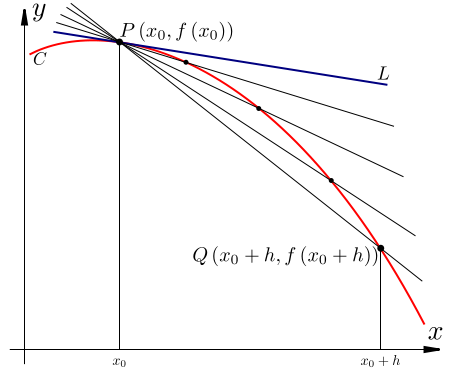
\includegraphics[width=1.8in]{Tangent_as_Secant_Limit.png}
     \caption{Secant lines between $P$ and $Q$, as $Q$ approaches $P$}
     \label{fig:4}
  \end{figure}
  }
  
\frame
{
\frametitle{Instantaneous rate of change}
\[ \text{Slope of the tangent line at }P = \lim_{h\to 0}\frac{f(x_0+h)-f(x_0)}{h}\]\pause
\begin{ex}
Find the instantaneous rate of change of $f(x)=4x-3x^2$ at $x=2$.\pause

\nin {\bf Solution:}\vspace*{-5mm}  \begin{eqnarray*}
\text{ Average rate of change }&=& \frac{f(x)-f(2)}{x-2} \\ 
&=& \frac{4x-3x^2-(4\cdot 2-3\cdot 2^2)}{x-2}\\ \pause
&=& \frac{(x-2)(-3x-2)}{x-2} = -3x-2
\end{eqnarray*}\pause
\vspace*{-4mm} \[\text{Instantaneous rate of change of }f(x)\text{ at }2\,=\lim_{x\to 2}-3x-2=-8.\]
\end{ex}
}

\frame
{
\frametitle{Definition of derivative}
\begin{dfn}
The derivative of a function $f(x)$, denoted $f'(x)$, gives at each point $a$, the value of the instantaneous rate of change of $f(x)$ at $x=a$.
That is, \[ f'(a)=\text{Instantaneous rate of change of }f(x)\text{ at }x=a.\]\pause
Mathematically,
\[ f'(x)=\lim_{h\to 0}\frac{f(x+h)-f(x)}{h}.\]
\end{dfn}
\begin{rem}
$f'(a)$ = Slope of the tangent line to $f(x)$ at the point $x=a$.
\end{rem}
}

\begin{frame}
\frametitle{Important example}

\noindent Suppose an object moves along a straight line according to the equation of motion $y = f(t)$, where $y$ is the displacement of the object from the origin at time $t$, then we call $f$ the \emph{position function} of the object.  The \emph{velocity} of the object at $t=a$ is defined to be the instantaneous rate of change of the position function when $t=a$.  The \emph{speed} of the object at $t=a$ is defined to be the absolute value of the velocity when $t=a$.\\

\noindent Suppose an arrow is shot upwards on the moon with a velocity of $58$ meters per second, then its height in meters after $t$ seconds is given by
\[H = 58t - 0.83t^{2}.\]
Find the velocity and speed of the arrow after $1$ second.
\end{frame}
 
\begin{frame}
\begin{ex}
Let's compute the derivative $f'$ of the function $f(x) = \sqrt{x}$ and find the domain.\end{ex}
\end{frame}


\frame
{
\frametitle{Equation of the tangent line}
\begin{ex}
Find the equation of the tangent line to the graph 
 $f(x)= x^2$ at $x=1$. \pause
 
 
\nin{\underline{\bf Solution:}} Apply the definition. The slope of the tangent line 
is given by\vspace*{-7mm} 
\[\begin{array}{lcl}
\disp{\lim_{h\to 0}} \dfrac{f(1+h)-f(1)}{h} &=& \disp{\lim_{h\to 0}} \dfrac{(1+h)^2- 1^2}{h}\\ \pause
&=& \disp{\lim_{h\to 0}} \dfrac{2h+h^2}{h}\\ \pause
&=& \disp{\lim_{h\to 0}}  (2+h) =2 \end{array}\] \pause
The tangent line to the graph 
 $f(x)= x^2$ at $x=1$ is a line through $(1, f(1))=(1, 1)$ with the slope $2$. \pause By the
 point-slope form, we get the equation of the tangent line,\vspace*{-4mm}
 \[
 y = 2(x-1) +1\Longrightarrow y= 2x-1.
 \]
 \end{ex}
 }

\subsection{Differentiable functions}
\begin{frame}
\begin{dfn} Suppose that $f$ is defined on some open interval containing the point $x$. We say that $f$ is \textit{differentiable} at $x$ if $f'(x)$ exists.\end{dfn}\pause

\newhead{Remark on notation} Other notation for $f'(x)$  includes $\frac{d}{dx}f(x)$ and $\frac{df}{dx}(x)$ . If $y=f(x)$ then the derivative is often denoted by $y'$ or $\frac{dy}{dx}$. The ratio
\[\frac{f(x+h)-f(x)}{h}\]
is called the \textit{difference quotient} for $f$ at the point $x$.\pause

\vspace*{.1cm}

\newhead{Example}

\noindent If $f(x) = |x|$, does $f'(0)$ exist?

\end{frame}

\begin{frame}
\begin{thm}
If $f$ is differentiable at $a$ then it is continuous at $a$. \end{thm}\pause

\vspace*{.4cm}

\noindent The converse of this theorem is \emph{false}.  There are functions (for instance $f(x) = |x|$) which are continuous at a point but not differentiable there.\pause

\noindent A function could fail to be differentiable for several reasons.   \pause
\begin{itemize}
\item The graph has a jump or a vertical tangent line, equivalently, the function is discontinuous. \pause
\item The graph has a sharp corner: the secant lines from the left and the right have different limits.
\end{itemize}

\end{frame}

\begin{frame}
\frametitle{Higher order derivatives}

\noindent If $f$ is a differentiable function with derivative $f'$, sometimes $f'$ may also be differentiable. If this is the case, then the derivative of $f'$ is denoted $f''$ and called the \textit{second derivative of $f$}.\pause If $y=f(x)$ then we can also write
\[f''(x)=\frac{d}{dx}\left(\frac{dy}{dx}\right)=\frac{d^2y}{dx^2}.\]\pause
If $f''$ is differentiable then its derivative $f'''$ is called the \textit{third\\ derivative of $f$}. The prime notation $f'''$ is only practical until the third derivative. For higher order derivatives we introduce new notation.
\end{frame}

\begin{frame}
\frametitle{Higher order derivatives}


\newhead{Notation} Suppose that $f$ can be differentiated $n$ times. Then its $n$th derivative is denoted by $f^{(n)}$. If $y=f(x)$ then we also write
\[f^{(n)}(x)=\frac{d^ny}{dx^n}.\]\pause

\noindent Higher order derivatives have various interpretations depending on the context. A geometric interpretation of the second derivative will be given in the next chapter. One interpretation that features in mechanics is that of \emph{acceleration}. As before, suppose that the position of a object that moves in a straight line is given by $y(t)$ at time $t$.  Then $v(t) = y'(t)$ is the velocity of the particle and $a(t) = v'(t)$ is its acceleration at time $t$.  Note that $a(t) = y''(t)$, so acceleration is the second derivative of position.
\end{frame}

\begin{frame}
\frametitle{Rules for differentiation}

\noindent So far we have calculated derivatives working directly from the definition, that is, by taking the limit as $h \to 0$ of the difference quotient. However, in practice this is often both difficult and tedious.  Luckily, there exist some nice rules that make it quite easy to compute the derivatives of most functions we are familiar with.

\newhead{Some basic derivatives}
\begin{center}
\begin{tabular}{|l|l|}
\hline
$f(x)$					& $f'(x)$			\\
\hline
$C$, where $C$ is a constant		& $0$				\\
$x^n$, where $n$ is a real number	& $nx^{n-1}$			\\
$\sin x$				& $\cos x$			\\
$\cos x$				& $-\sin x$		\\
$e^x$				& $e^x$ \\
$\ln x$				& $1/x$\\
\hline
\end{tabular}
\end{center}
\end{frame}

\end{document}